% \section*{Выбор средст программирования}

% Среда разработки: VS Codium version 1.78.2.

% Операционная система: Windows 10 version 22H2 OS Build 19045.2965.

% Эмулятор Android: Pixel 2 API 30 (Android 11.0 Google Play | x86).

% Версия NodeJS: NodeJS version 18.16.0.

\subsection{Результаты испытания мобильного приложения}

Среда тестирования - эмулятор Android Pixel 2 API 30 (Android 11.0 Google Play | x86)
на персональном компьютере HP model 15s-eq2025ur (Windows 10 Home, AMD Ryzen 3 5300U with Radeon Graphics, 8.00 GB RAM, 64-bit Operation System).


\subsubsection*{Тест 1: Ввод данных в форму регистрации}

Ожидаемый результат: при не введеном поле, мобильно приложение сообщит о незаполненом поле, иначе переходим на следующий этап.

Этапы регистрации:
\begin{itemize}
    \item[-] ввод УНП;
    \item[-] подтверждение данных своей организации по указаному УНП;
    \item[-] ввод даных представителя (ФИО, телефон приемной);
    \item[-] ввод данных аккаунта (логин, e-mail, пароль);
    \item[-] подтверждение аккаунта по электронной почте.
\end{itemize}

Если пользователь не укажет данные в как-то из полей, то мобильное приложение не даст перейти на следующий этап
и появится уведомление.
Исключением может быть поле <<Отчество>>, так как не у всех оно есть.
Поле <<Отчество>> можно не заполнять.

После ввода УНП данные, а именно полное наименование юридического лица, краткое наименование юридического лица, адрес
подтягиваются с сайта portal.nalog.gov.by (см. рисунок~\ref{fig:test_registration_step1}).
Если пользователь убеждается в правильности ввода УНП, то переходит на следующий этап.

\begin{figure}[!htb]\centering
    \begin{minipage}{0.19\textwidth}
        \centering

        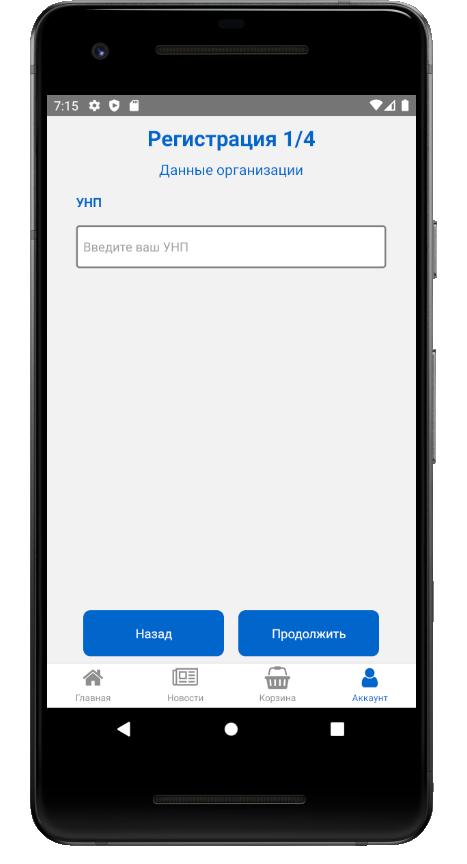
\includegraphics[height=5cm]
        {images/mobile/registration/step1.png}
    \end{minipage}
    \begin{minipage}{0.19\textwidth}
        \centering

        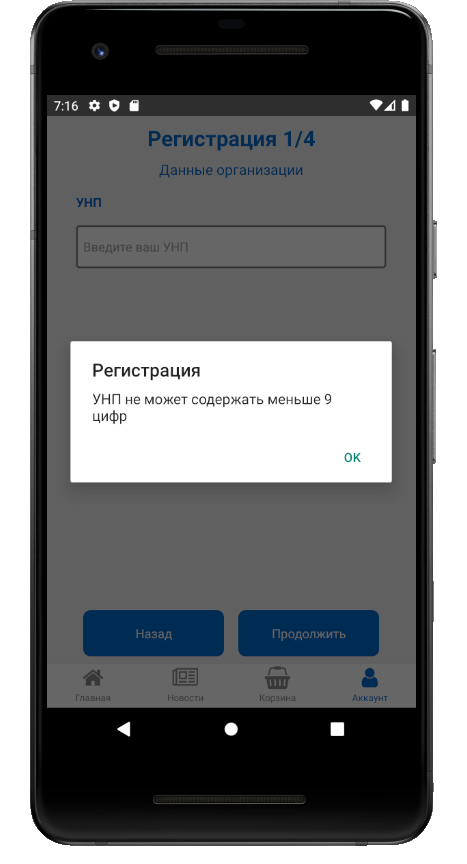
\includegraphics[height=5cm]
        {images/mobile/registration/unp.png}
    \end{minipage}
    \begin{minipage}{0.19\textwidth}
        \centering

        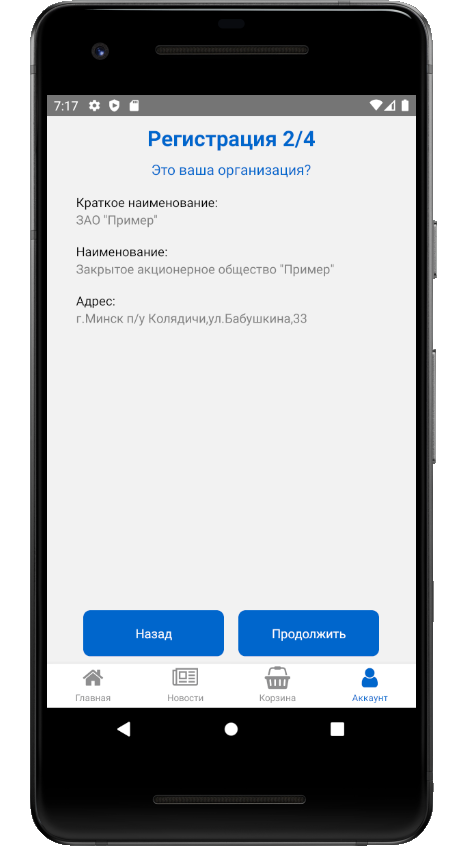
\includegraphics[height=5cm]
        {images/mobile/registration/step2.png}
    \end{minipage}
  
    \caption{Регистрация этап 1 и 2}
    \label{fig:test_registration_step1}
\end{figure}

\begin{figure}[!htb]\centering
    \begin{minipage}{0.19\textwidth}
        \centering

        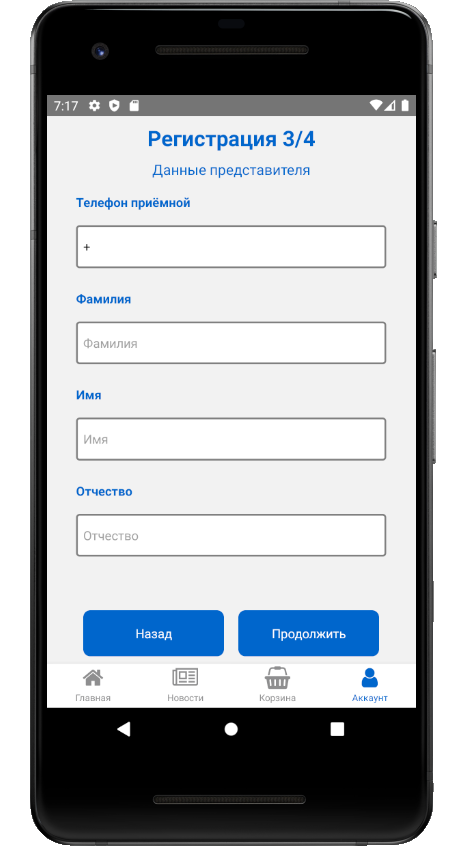
\includegraphics[height=5cm]
        {images/mobile/registration/step3.png}
    \end{minipage}
    \begin{minipage}{0.19\textwidth}
        \centering

        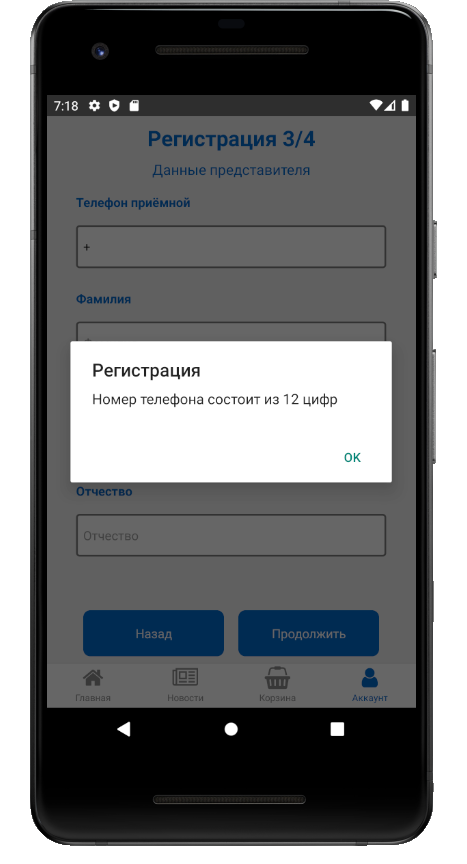
\includegraphics[height=5cm]
        {images/mobile/registration/phone.png}
    \end{minipage}
    \begin{minipage}{0.19\textwidth}
        \centering

        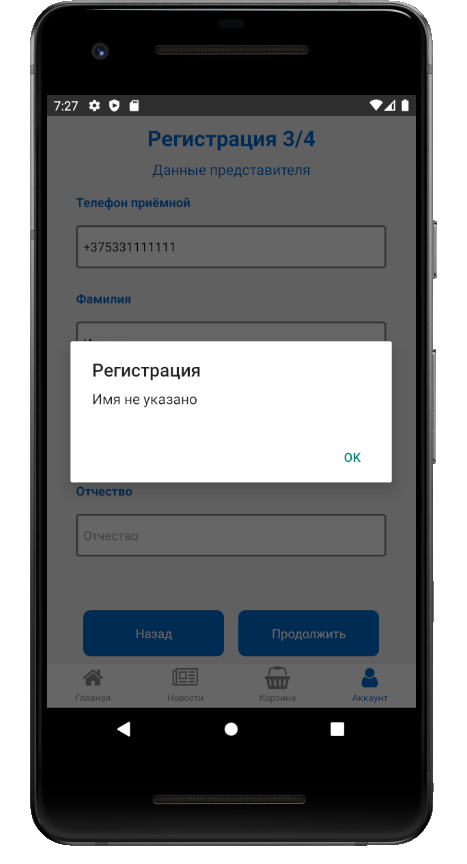
\includegraphics[height=5cm]
        {images/mobile/registration/name.png}
    \end{minipage}
    \begin{minipage}{0.19\textwidth}
        \centering

        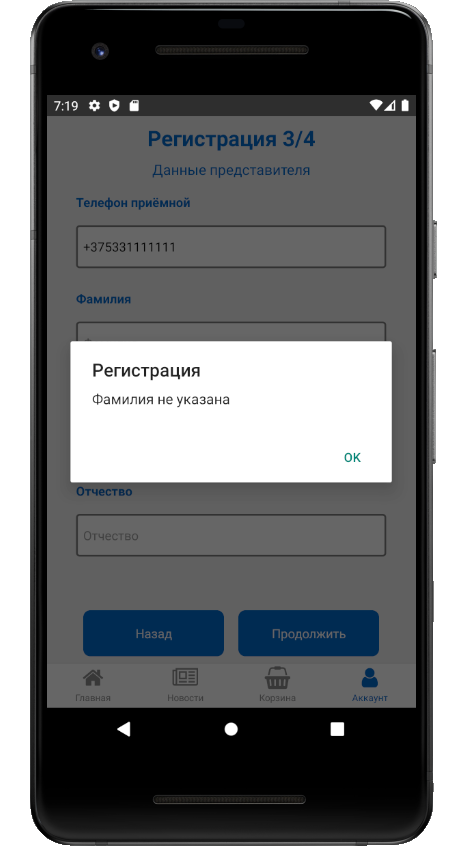
\includegraphics[height=5cm]
        {images/mobile/registration/surname.png}
    \end{minipage}
    % \begin{minipage}{0.19\textwidth}
    %     \centering

    %     \includegraphics[height=5cm]
    %     {images/mobile/registration/step1.png}
    % \end{minipage}

    \caption{Регистрация этап 3}
    \label{fig:test_registration_step3}
\end{figure}

\begin{figure}[!htb]\centering
    \begin{minipage}{0.19\textwidth}
        \centering

        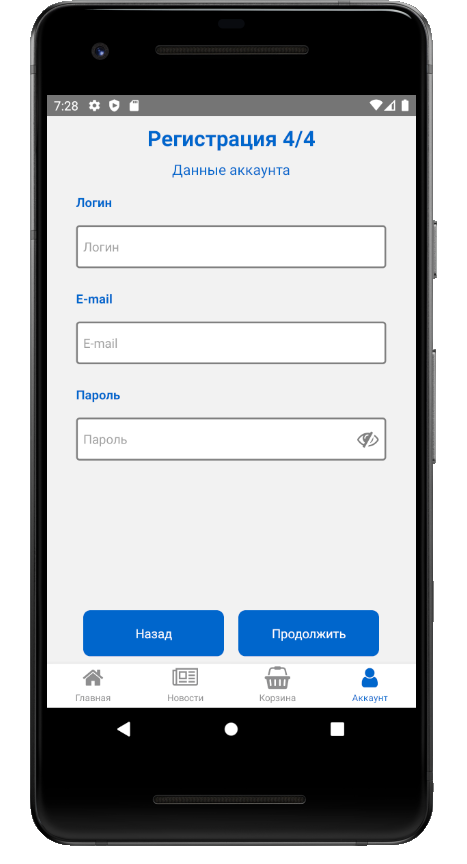
\includegraphics[height=6cm]
        {images/mobile/registration/step4.png}
    \end{minipage}
    \begin{minipage}{0.19\textwidth}
        \centering

        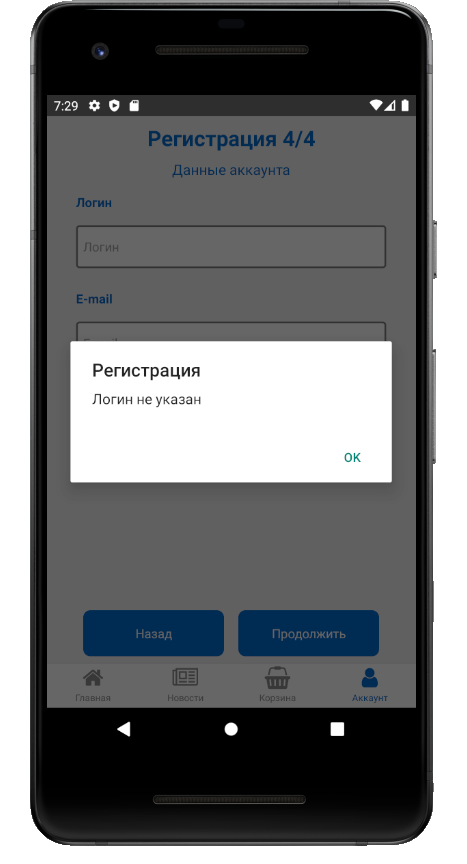
\includegraphics[height=6cm]
        {images/mobile/registration/login.png}
    \end{minipage}
    \begin{minipage}{0.19\textwidth}
        \centering

        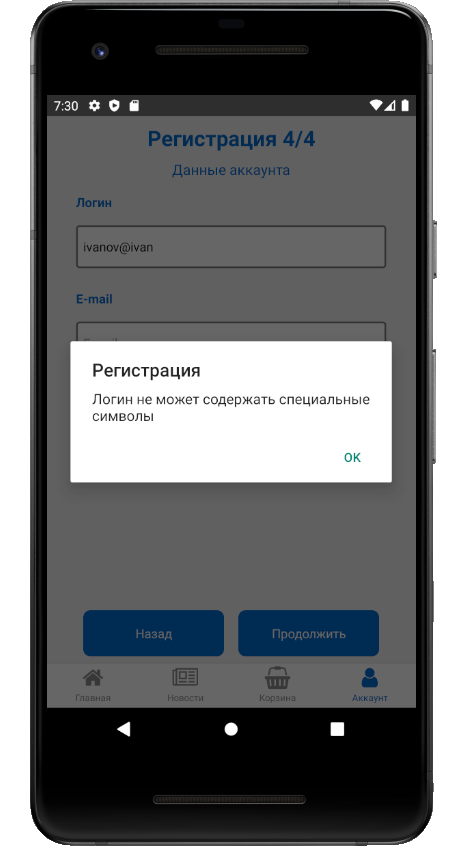
\includegraphics[height=6cm]
        {images/mobile/registration/login_special.png}
    \end{minipage}
    \begin{minipage}{0.19\textwidth}
        \centering

        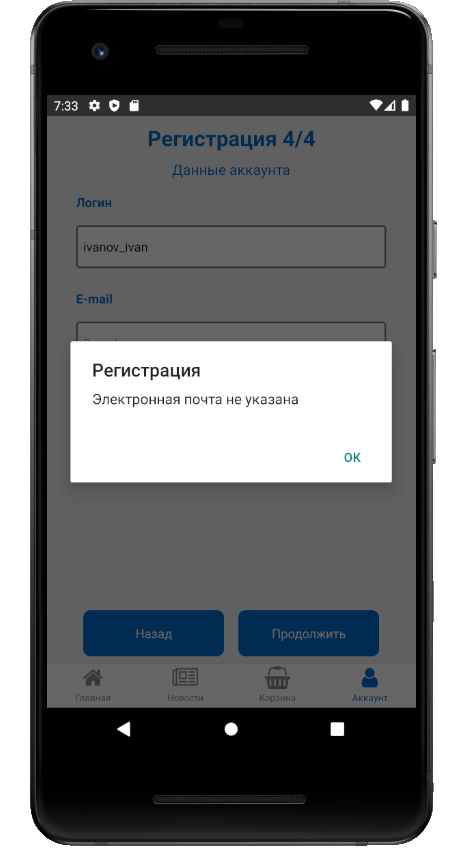
\includegraphics[height=6cm]
        {images/mobile/registration/email.png}
    \end{minipage}
    \begin{minipage}{0.19\textwidth}
        \centering

        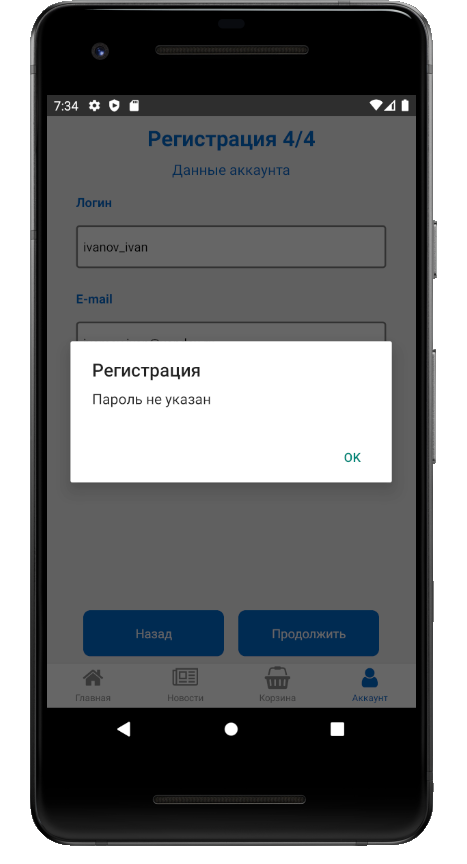
\includegraphics[height=6cm]
        {images/mobile/registration/password.png}
    \end{minipage}

    \caption{Регистрация этап 4}
    \label{fig:test_registration_step4}
\end{figure}

\begin{figure}[!htb]\centering
    \begin{minipage}{0.19\textwidth}
        \centering

        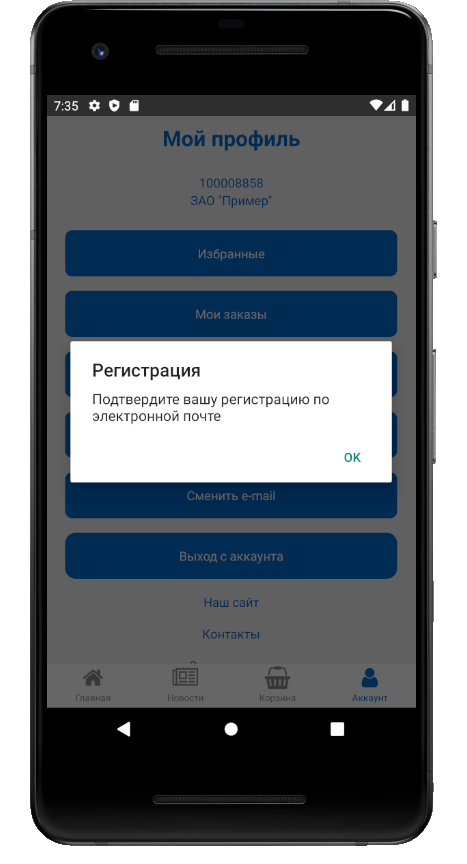
\includegraphics[height=6cm]
        {images/mobile/registration/finish.png}
    \end{minipage}
    \begin{minipage}{0.19\textwidth}
        \centering

        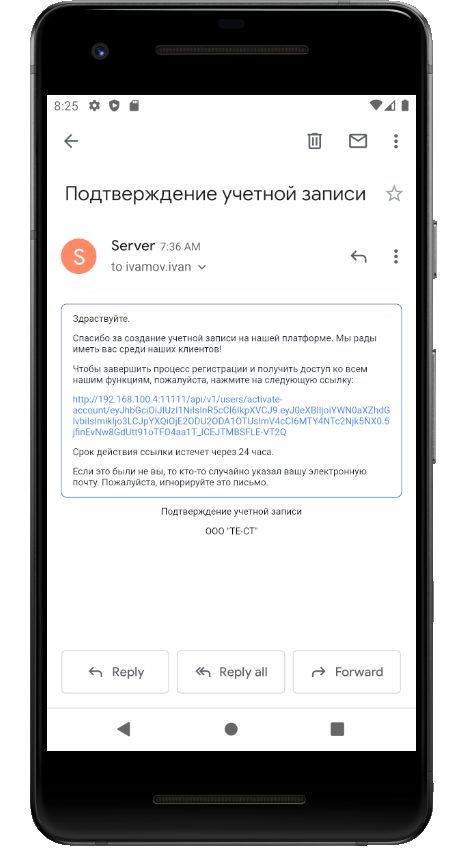
\includegraphics[height=6cm]
        {images/mobile/registration/activation.png}
    \end{minipage}
    \begin{minipage}{0.19\textwidth}
        \centering

        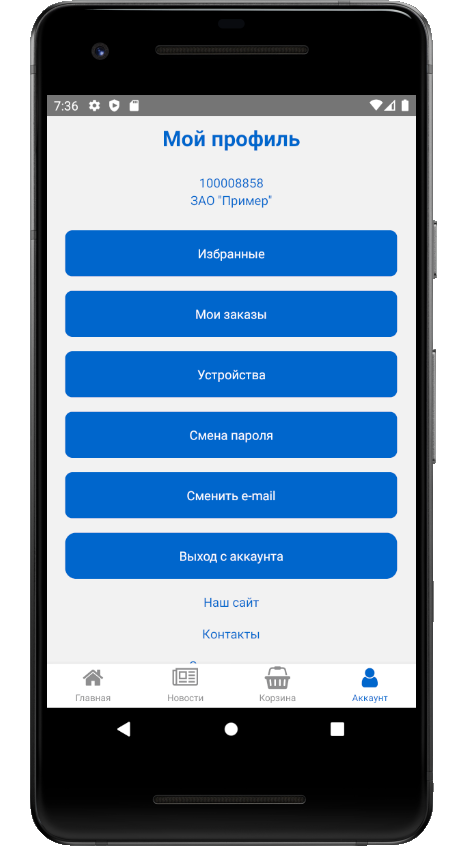
\includegraphics[height=6cm]
        {images/mobile/registration/finish_account.png}
    \end{minipage}
    
    \caption{Конец регистрации}
    \label{fig:test_registration_step4}
\end{figure}

Вывод: проверены все текстовые поля на их незаполнение, при пропуске ввода поля мобильное приложение сообщает о необходимости его заполнения, регистрация работает корректно.


\subsubsection*{Тест 2: Отображение данных о номенклатуре при интернете}

Ожидаемый результат: при подключенном интернете будут подтягиваться данные о номенклатуре из базы данных (см. рисунок~\ref{fig:test_internet_items}),
иначе пустой экран с текстом <<Протяните вниз для обновления>>
c всплывающим уведомлением на секунду об отсутвии интернета.

\begin{figure}[!htb]\centering
    \begin{minipage}{0.16\textwidth}
        \centering

        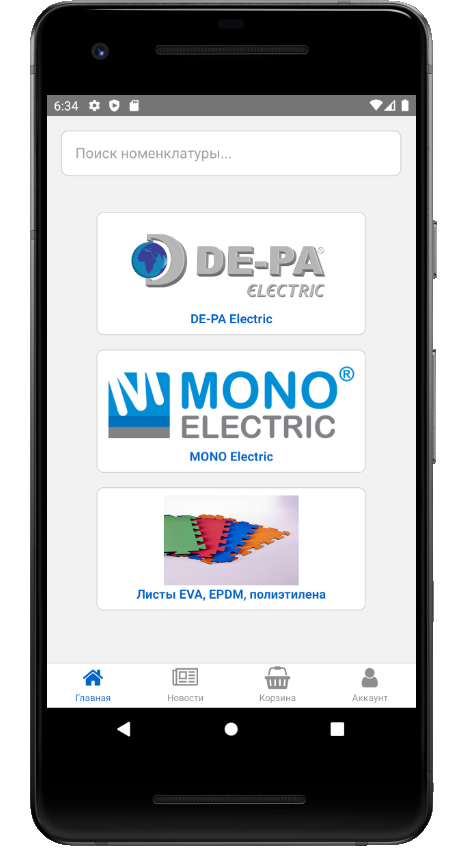
\includegraphics[height=5.8cm]
        {images/mobile/items/item-brands.png}
    \end{minipage}
    \begin{minipage}{0.16\textwidth}
        \centering

        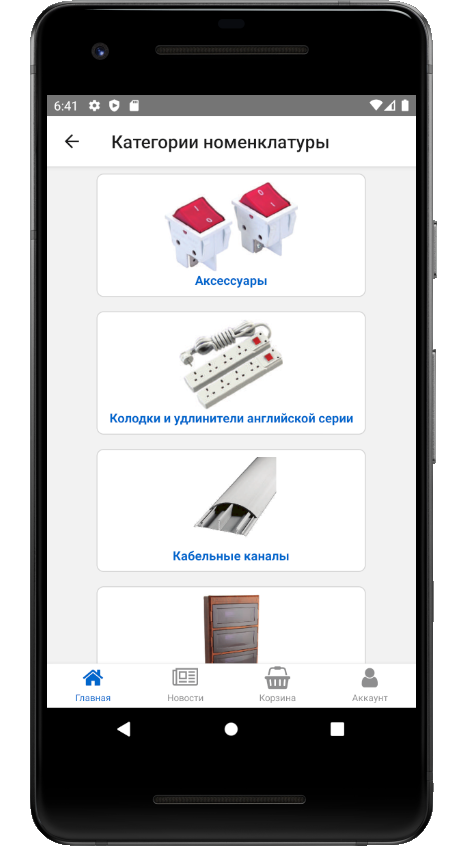
\includegraphics[height=5.8cm]
        {images/mobile/items/item-categories.png}
    \end{minipage}
    \begin{minipage}{0.16\textwidth}
        \centering

        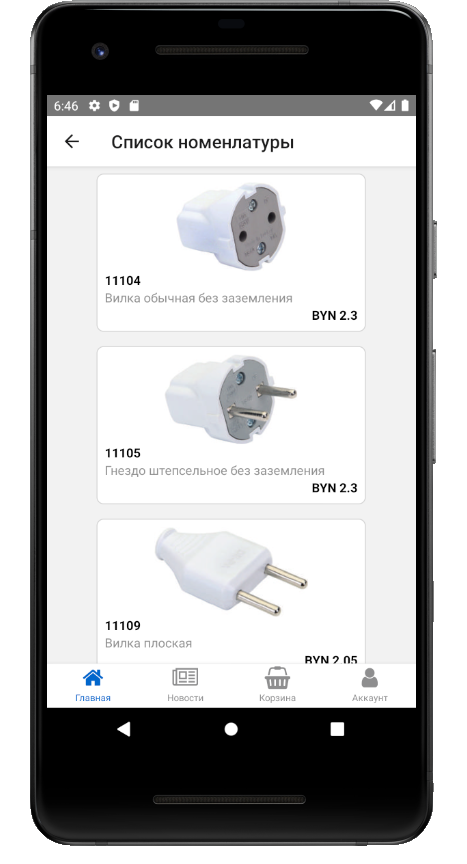
\includegraphics[height=5.8cm]
        {images/mobile/items/items.png}
    \end{minipage}
    \begin{minipage}{0.16\textwidth}
        \centering

        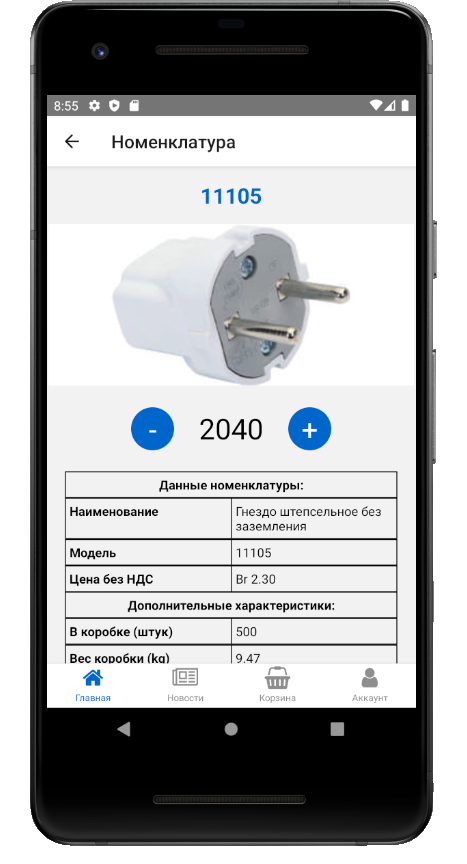
\includegraphics[height=5.8cm]
        {images/mobile/items/item.png}
    \end{minipage}
    \begin{minipage}{0.16\textwidth}
        \centering

        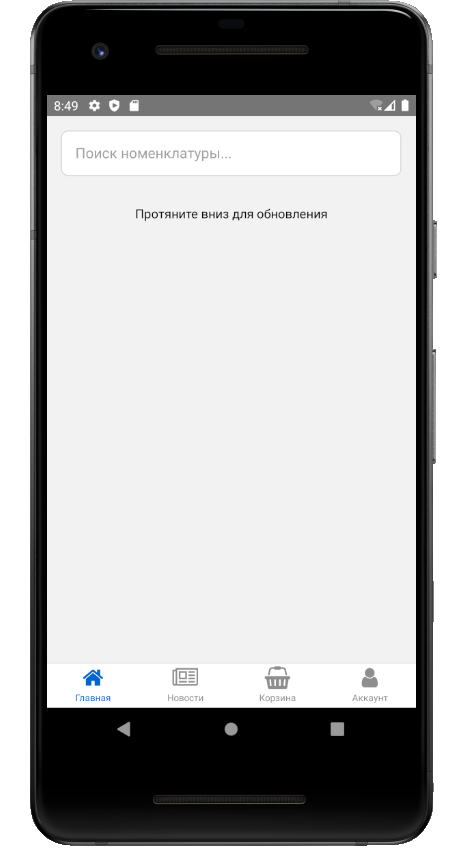
\includegraphics[height=5.8cm]
        {images/mobile/items/no-internet.png}
    \end{minipage}
    \begin{minipage}{0.16\textwidth}
        \centering

        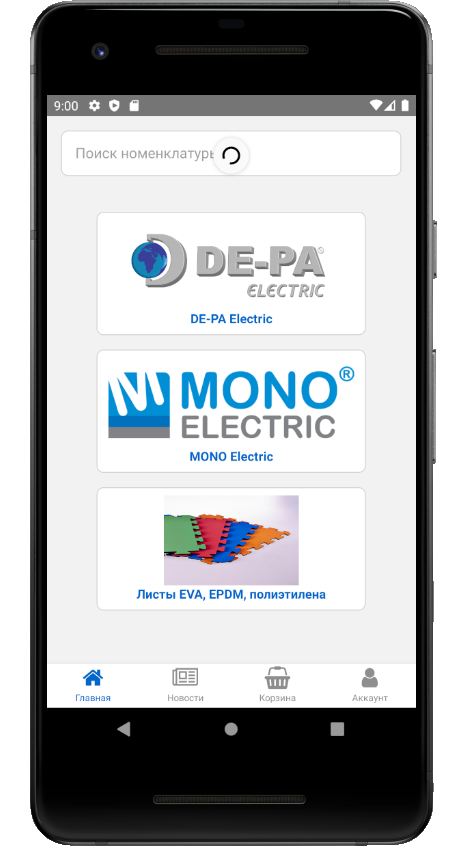
\includegraphics[height=5.8cm]
        {images/mobile/items/spin.png}
    \end{minipage}
  
    \caption{Отображение номенклатуры с и без интернета}
    \label{fig:test_internet_items}
\end{figure}

Вывод: при подключенном интернете появляется на секунду надпись <<Нет доступа к интернету...>>.
Для обновления записей можно протянуть пальцем вниз. Если нет достпа в интернет,
то кружочек перестанет крутится и появится на секунду надпись <<Нет доступа к интернету...>>.
Если при открытиии мобильного приложения не было интернета и оно не успело загрузить какие-то данные, то будет пустой экран с надписью
<<Протяните вниз для обновления>>.

\subsubsection*{Тест 3: Отображение данных о статьях при интернете}

Ожидаемый результат: при подключенном интернете будут подтягиваться данные о статьях из базы данных (см. рисунок~\ref{fig:test_internet_articles}),
иначе пустой экран с текстом <<Протяните вниз для обновления>>
c всплывающим уведомлением на секунду об отсутвии интернета.

\begin{figure}[!htb]\centering
    \begin{minipage}{0.16\textwidth}
        \centering

        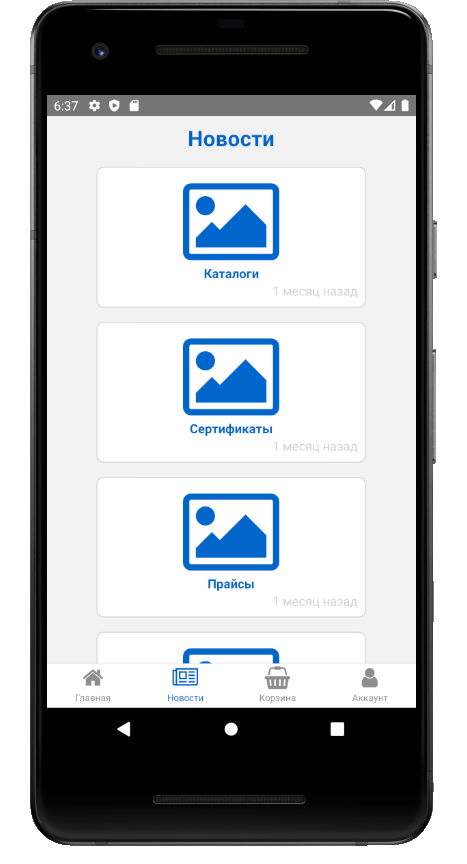
\includegraphics[height=5.8cm]
        {images/mobile/articles/articles.png}
    \end{minipage}
    \begin{minipage}{0.16\textwidth}
        \centering

        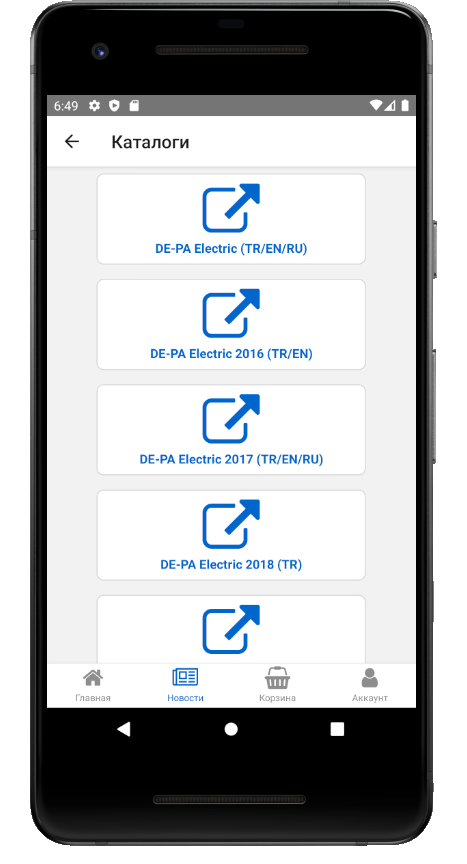
\includegraphics[height=5.8cm]
        {images/mobile/articles/article_catalogs.png}
    \end{minipage}
    \begin{minipage}{0.16\textwidth}
        \centering

        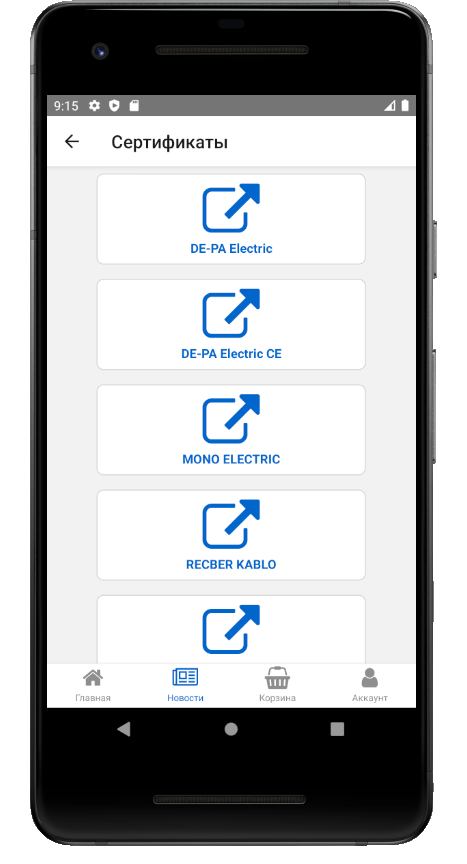
\includegraphics[height=5.8cm]
        {images/mobile/articles/article_certificates.png}
    \end{minipage}
    \begin{minipage}{0.16\textwidth}
        \centering

        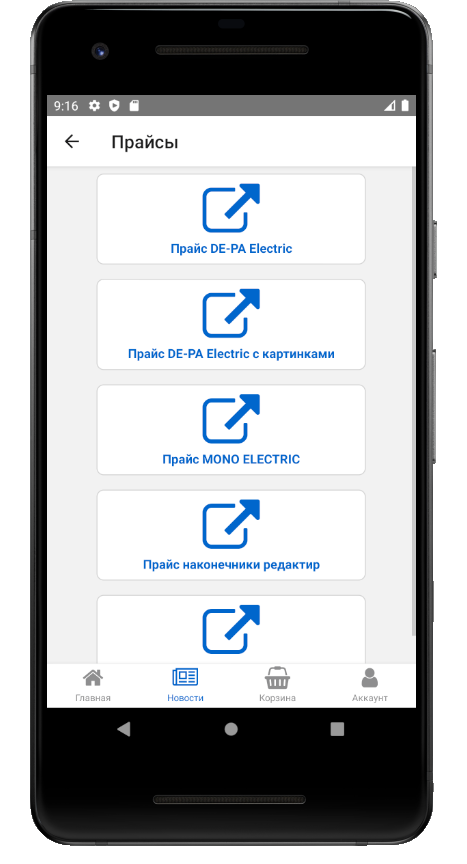
\includegraphics[height=5.8cm]
        {images/mobile/articles/article_prices.png}
    \end{minipage}
    \begin{minipage}{0.16\textwidth}
        \centering

        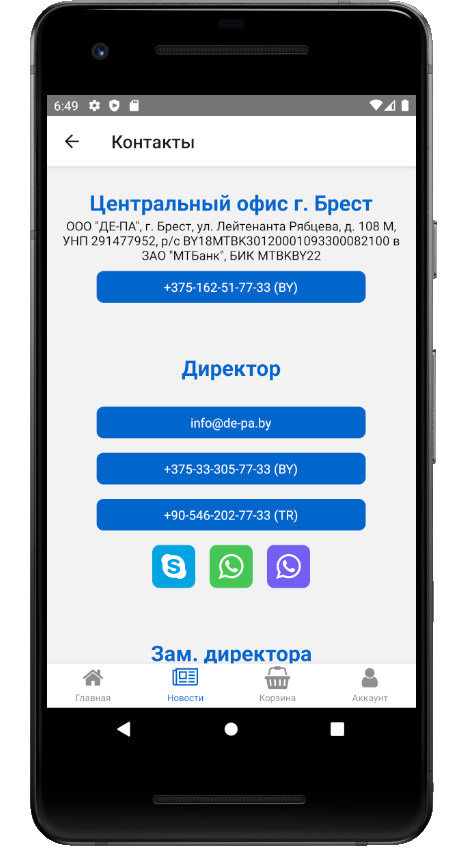
\includegraphics[height=5.8cm]
        {images/mobile/articles/article_contacts.png}
    \end{minipage}
    \begin{minipage}{0.16\textwidth}
        \centering

        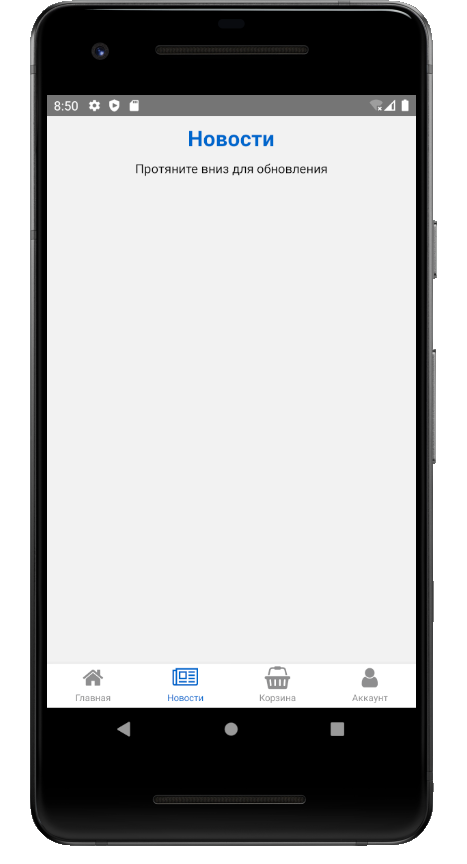
\includegraphics[height=5.8cm]
        {images/mobile/articles/no-internet.png}
    \end{minipage}
  
    \caption{Отображение статей с и без интернета}
    \label{fig:test_internet_articles}
\end{figure}

Вывод: при подключенном интернете появляется на секунду надпись <<Нет доступа к интернету...>>.
Для обновления записей можно протянуть пальцем вниз. Если нет достпа в интернет,
то кружочек перестанет крутится и появится на секунду надпись <<Нет доступа к интернету...>>.
Если при открытиии мобильного приложения не было интернета и оно не успело загрузить какие-то данные, то будет пустой экран с надписью
<<Протяните вниз для обновления>>.

\subsubsection*{Тест 4: Добавление в избранное только авторизованному пользователю}

Ожидаемый результат: если пользователь авторизован (см. рисунок~\ref{fig:test_like_items}), то он может добавить номенклатуру в избранные
(синей значок <<сердечко>> - номенклатура добавлена в избранные,
серый значок <<сердечко>> - номенклатуры не в списке избранных),
иначе, если пользователь не авторизован, иконок <<сердечко>> нет (см. рисунок~\ref{fig:test_nolike_items}).

\begin{figure}[!htb]\centering
    \begin{minipage}{0.49\textwidth}
        \centering

        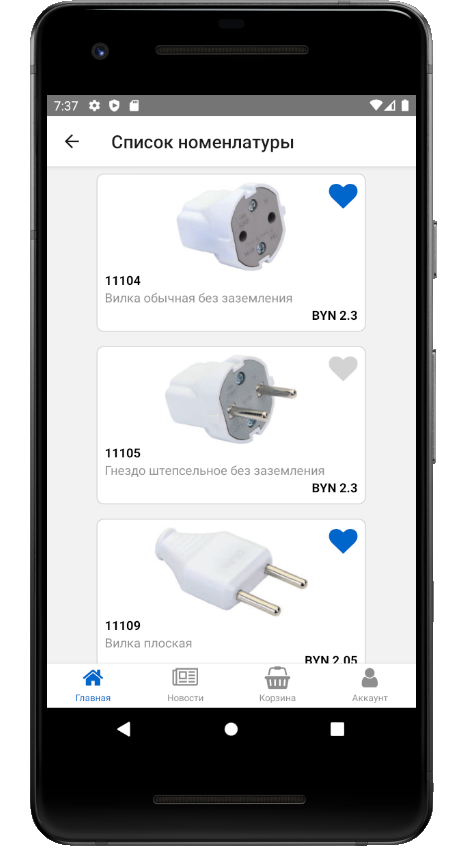
\includegraphics[height=9.2cm]
        {images/mobile/items/items_with_account.png}

        \caption{Номенклатура c иконками <<сердечко>>}
        \label{fig:test_like_items}
    \end{minipage}
    \begin{minipage}{0.49\textwidth}
        \centering

        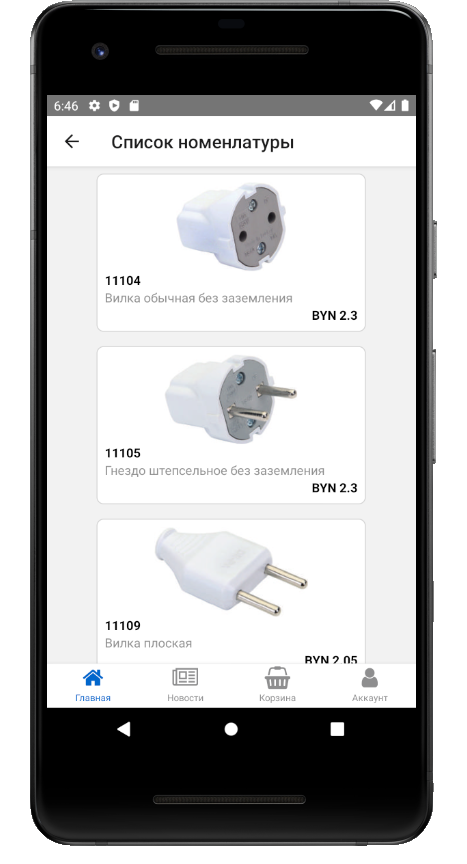
\includegraphics[height=9.2cm]
        {images/mobile/items/items.png}

        \caption{Номенклатура без иконок <<сердечко>>}
        \label{fig:test_nolike_items}
    \end{minipage}
\end{figure}

Список избранных в отличии от корзины хранится в базе данных.
Если пользователь не авторизован, то он лишается возможности добавлять номенклатуру в список избранных.

Авторизованный пользователь и не авторизованный мользователь могут добавлять номенклатуру в корзину.
Корзина не хранится в базе данных удаленно. Корзина хранится на устройстве пользователя.

Вывод: если пользователь вошел в аккаунт, то отображаются иконки <<сердечко>> для добавления номенклатуры в избранное.
Добавление в избранные номенклатуры работает корректно.

\subsubsection*{Тест 5: Просмотр и закрытие сессии}

Ожидаемый результат:
\begin{itemize}
    \item[-] при завершении одной сессии - сессия завершается и список сессий обновляется (см. рисунок~\ref{fig:test_sessions_close_one});
    \item[-] при завершении всех сессий - все сессия закрываются и выбрасывает на экран входа (см. рисунок~\ref{fig:test_sessions_close_all}).
\end{itemize}

\begin{figure}[!htb]\centering
    \begin{minipage}{0.19\textwidth}
        \centering

        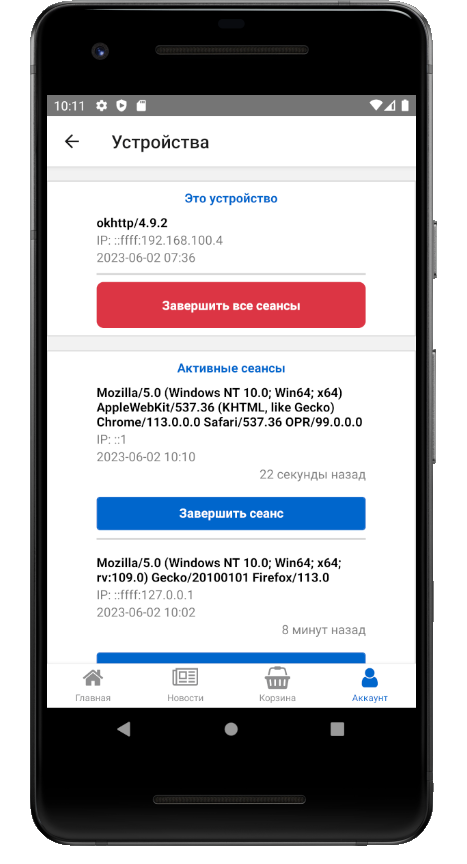
\includegraphics[height=7cm]
        {images/mobile/sessions/sessions.png}
    \end{minipage}
    \begin{minipage}{0.19\textwidth}
        \centering

        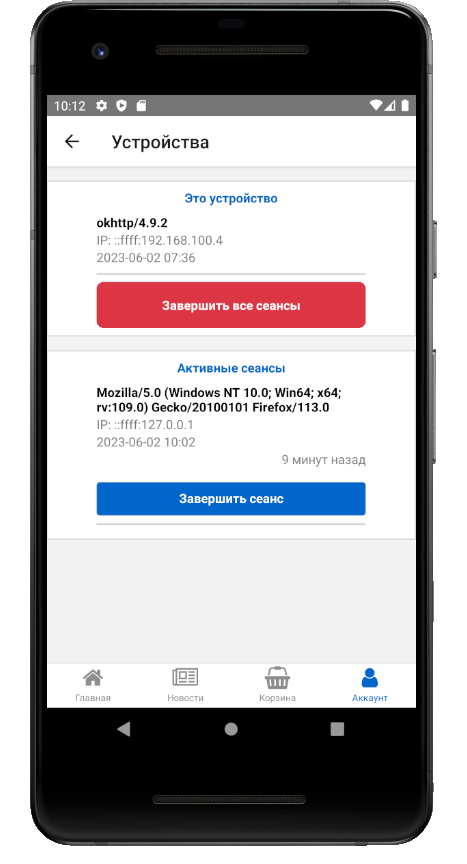
\includegraphics[height=7cm]
        {images/mobile/sessions/sessions_close_one.png}
    \end{minipage}

    \caption{До и после закрытия одной сессии}
    \label{fig:test_sessions_close_one}
\end{figure}

\begin{figure}[!htb]\centering
    \begin{minipage}{0.19\textwidth}
        \centering

        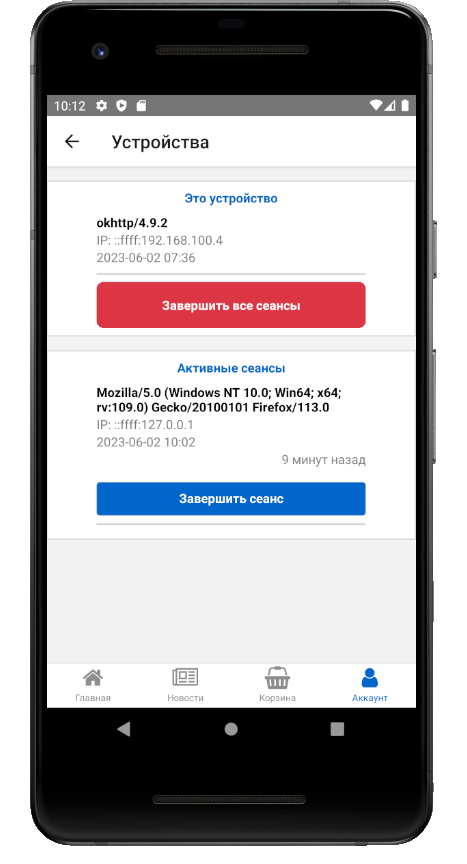
\includegraphics[height=7.2cm]
        {images/mobile/sessions/sessions_close_one.png}
    \end{minipage}
    \begin{minipage}{0.19\textwidth}
        \centering

        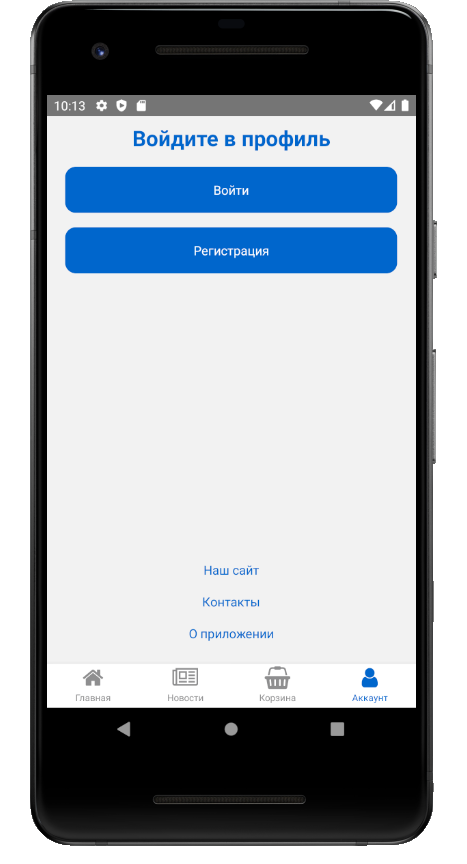
\includegraphics[height=7.2cm]
        {images/mobile/sessions/sessions_close_all.png}
    \end{minipage}
    \begin{minipage}{0.19\textwidth}
        \centering

        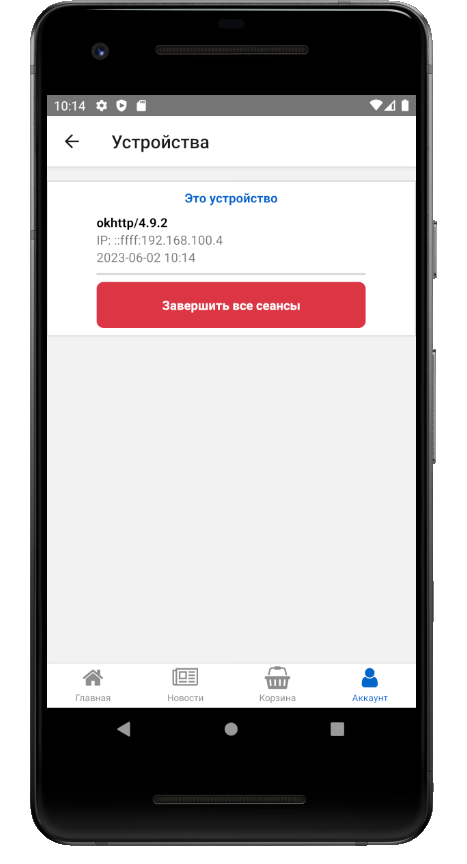
\includegraphics[height=7.2cm]
        {images/mobile/sessions/sessions_after_close_all.png}
    \end{minipage}

    \caption{До и после закрытия всех сессий}
    \label{fig:test_sessions_close_all}
\end{figure}

Вывод:
\begin{itemize}
    \item[-] завершение одной сессии работает корректно, сессия завершалась и список сессий обновился;
    \item[-] завершение всех сессий работает корректно, все сессии закрылись и выбрасило на экран входа,
    после авторизации заметили пустой список сессий, с сессией с текущим временем (было время 07:36, стало 10:14).
\end{itemize}

\subsubsection*{Тест 6: Выход из аккаунта}

Ожидаемый результат: после нажатия кнопки <<Выход из аккаунта>> закроется только текущаяя сессия (см. рисунок~\ref{fig:test_logout}).

\begin{figure}[!htb]\centering
    \begin{minipage}{0.19\textwidth}
        \centering

        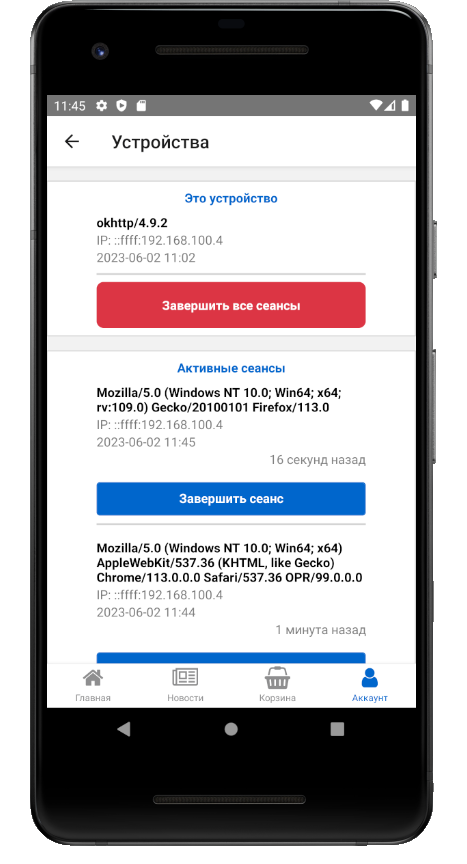
\includegraphics[height=7.2cm]
        {images/mobile/logout/sessions_before.png}
    \end{minipage}
    \begin{minipage}{0.19\textwidth}
        \centering

        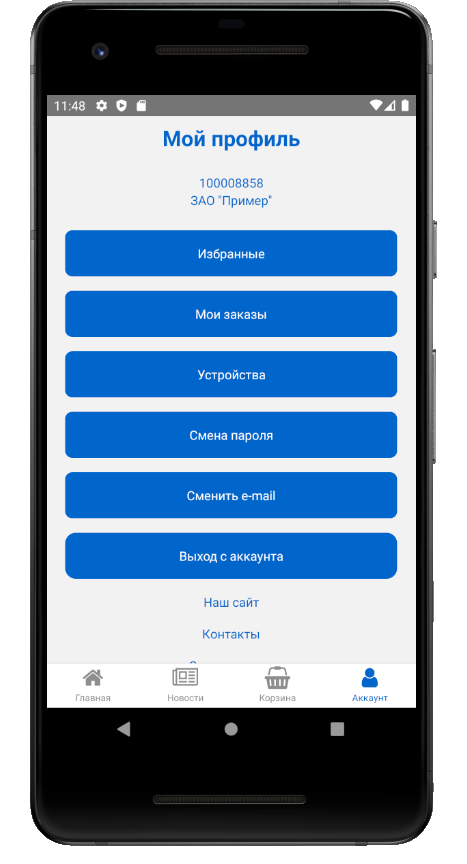
\includegraphics[height=7.2cm]
        {images/mobile/logout/logout_button.png}
    \end{minipage}
    \begin{minipage}{0.19\textwidth}
        \centering

        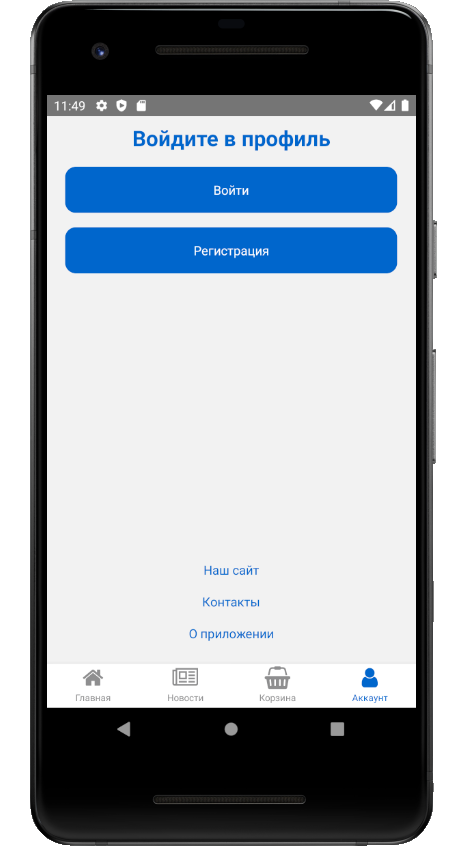
\includegraphics[height=7.2cm]
        {images/mobile/logout/login_page.png}
    \end{minipage}
    \begin{minipage}{0.19\textwidth}
        \centering

        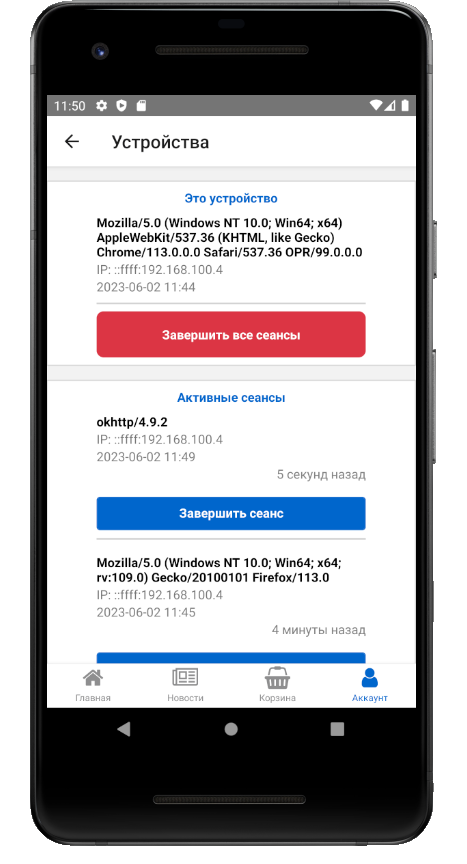
\includegraphics[height=7.2cm]
        {images/mobile/logout/sessions_after.png}
    \end{minipage}

    \caption{Выход из аккаунта}
    \label{fig:test_logout}
\end{figure}

Вывод:
после нажатия кнопки <<Выход из аккаунта>> выбрасило на страницу входа в аккаунт, а после входа
на странице <<Устройства>> было замечено новое время (было 10:04, стало 11:02) и оставшие два сеанса
(третьего сеанса с временем 10:04 не было). Выход из аккаунта работает корректно.

\subsubsection*{Тест 7: Добавление товара в корзину}

Ожидаемый результат: после добавление товара к корзину на странице <<Корзина>> появится список номенклатуры (см. рисунок~\ref{fig:test_basket}).

\begin{figure}[!htb]\centering
    \begin{minipage}{0.32\textwidth}
        \centering

        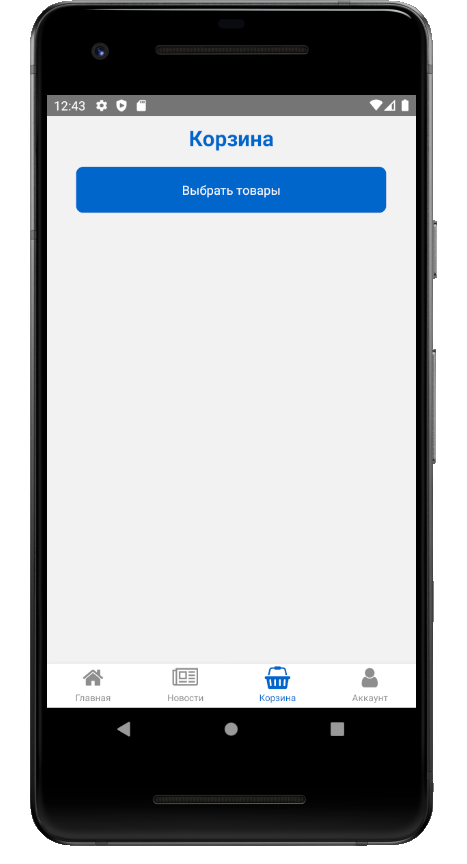
\includegraphics[height=7cm]
        {images/mobile/basket/basket_0.png}
    \end{minipage}
    \begin{minipage}{0.32\textwidth}
        \centering

        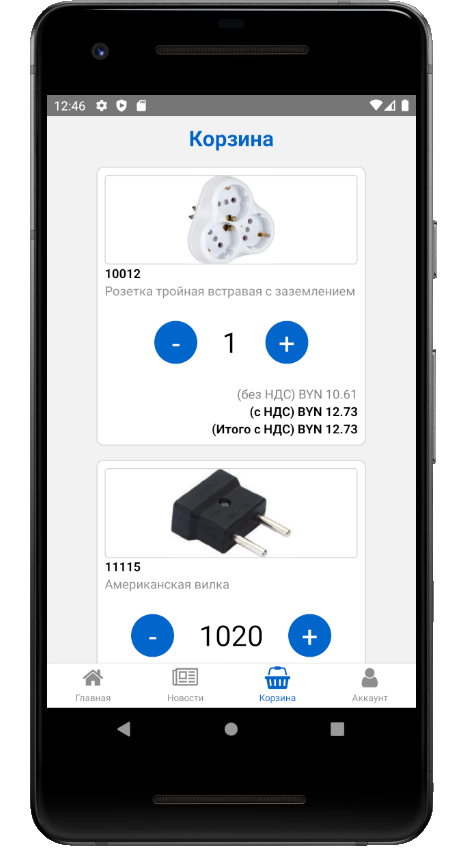
\includegraphics[height=7cm]
        {images/mobile/basket/basket_5.png}
    \end{minipage}

    \caption{До и после добавления номенклатуры в корзину}
    \label{fig:test_basket}
\end{figure}

Есть два спосаба редактирование номенклатуры:
\begin{itemize}
    \item[-] через кнопки <<+>> и <<->> (см. рисунок~\ref{fig:test_basket_plus_minus});
    \item[-] через числовую клавиатуру (см. рисунок~\ref{fig:test_basket_keyboard}).
\end{itemize}

\begin{figure}[!htb]\centering
    \begin{minipage}{0.49\textwidth}\centering
        \begin{minipage}{0.40\textwidth}
            \centering
    
            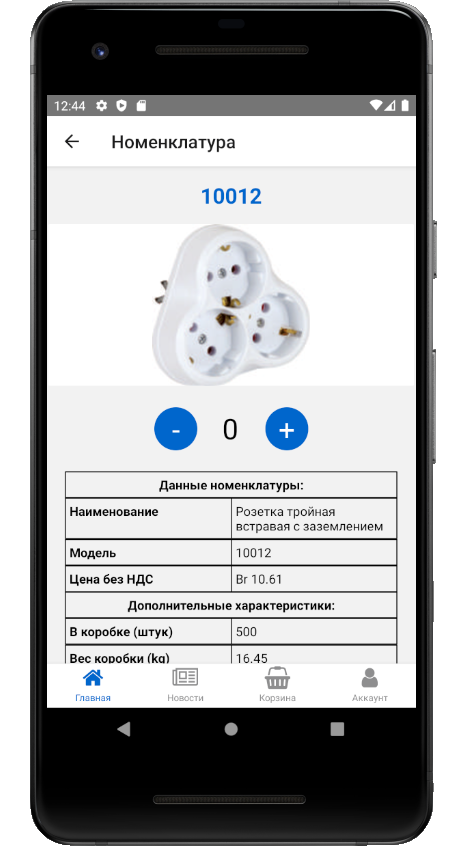
\includegraphics[height=7cm]
            {images/mobile/basket/basket_1.png}
        \end{minipage}
        \begin{minipage}{0.33\textwidth}
            \centering
    
            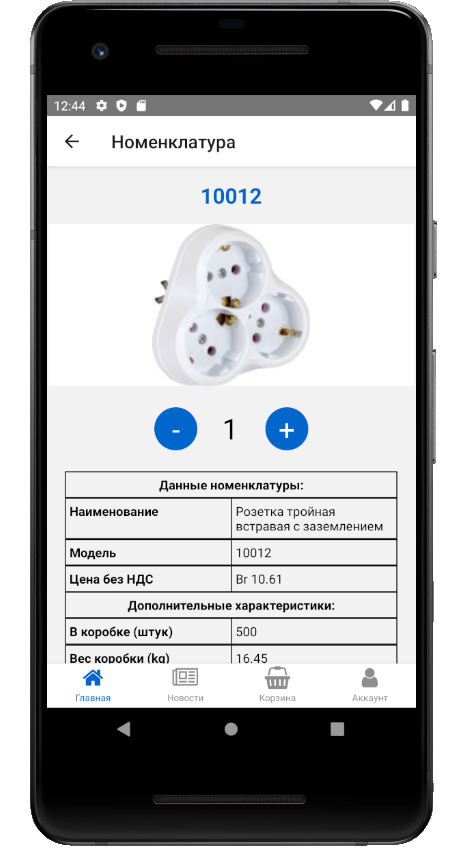
\includegraphics[height=7cm]
            {images/mobile/basket/basket_2.png}
        \end{minipage}

        \caption{Добавление номенклатуры в корзину кнопкой <<+>>}
        \label{fig:test_basket_plus_minus}
    \end{minipage}
    \begin{minipage}{0.49\textwidth}\centering
        \begin{minipage}{0.40\textwidth}
            \centering
    
            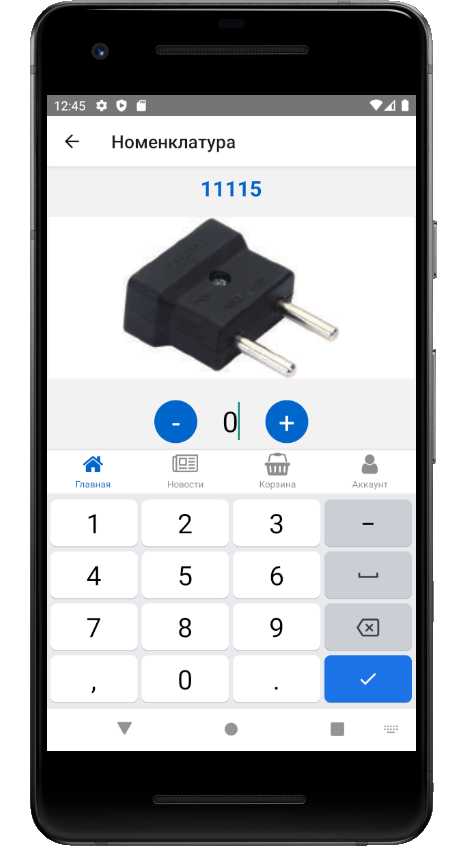
\includegraphics[height=7cm]
            {images/mobile/basket/basket_3.png}
        \end{minipage}
        \begin{minipage}{0.40\textwidth}
            \centering
    
            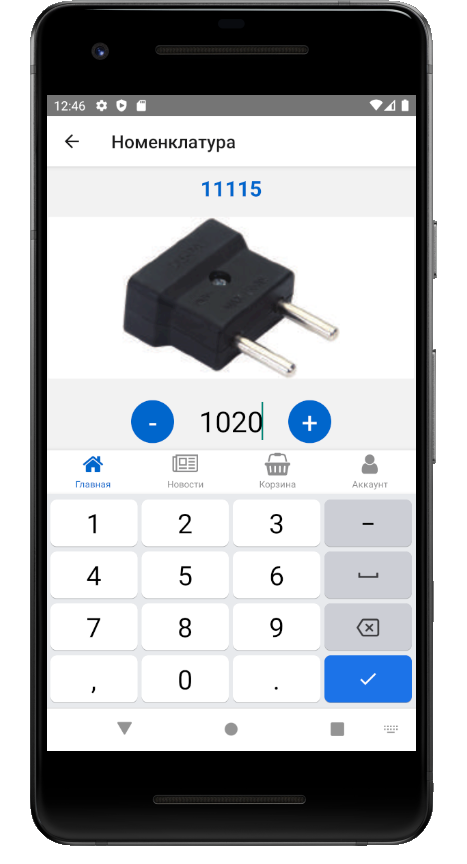
\includegraphics[height=7cm]
            {images/mobile/basket/basket_4.png}
        \end{minipage}

        \caption{Добавление номенклатуры в корзину клавиатурой}
        \label{fig:test_basket_keyboard}
    \end{minipage}   
\end{figure}

Вывод: при изменении количества единиц номенклатуры как через кнопку <<+>>, так и через клавиатуру, изменения применеются к корзине корректно.

\subsubsection*{Тест 8: Оформление заказа}

Ожидаемый результат:

\begin{itemize}
    \item[-] если сообщение отправлено менеджеру и клиенту,
    то корзина очищается и выскакиет сообщение об отправке документа <<Счёт-фактура>> (см. рисунок~\ref{fig:test_order_make});
    \item[-] если клиент заполняет поля для документа <<Счёт-фактура>>;
    то при его запросе должно выскочить уведомление об не заполненом поле (см. рисунок~\ref{fig:test_order_check});
    \item[-] в случает успеха отправки заявки должно прийти сообщение на электронную почту (см. рисунок~\ref{fig:test_order_check});
    \item[-] в случае успеха отправки документа <<Счёт-фактура>> на электронную почту должно прийти сообщение (см. рисунок~\ref{fig:test_order_check})
    с прикрепленным Excel документом (см. рисунок~\ref{fig:test_order_excel}).
\end{itemize}

\begin{figure}[!htb]\centering
    \begin{minipage}{0.24\textwidth}
        \centering

        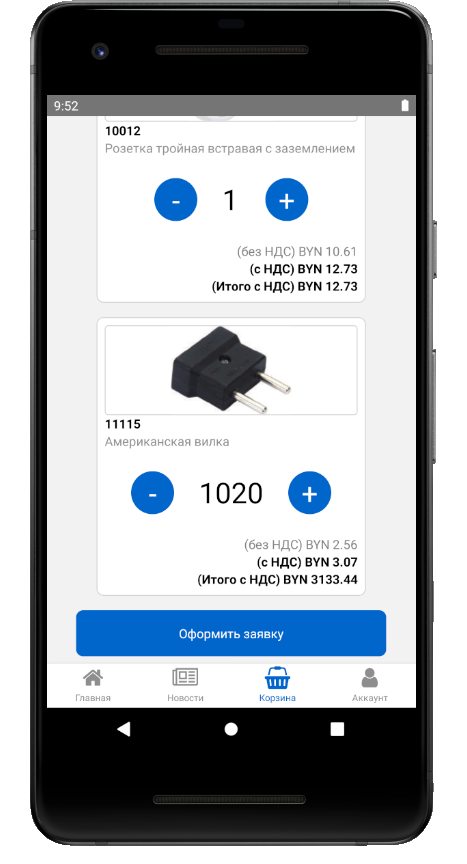
\includegraphics[height=6cm]
        {images/mobile/order/basket.png}
    \end{minipage}
    \begin{minipage}{0.24\textwidth}
        \centering

        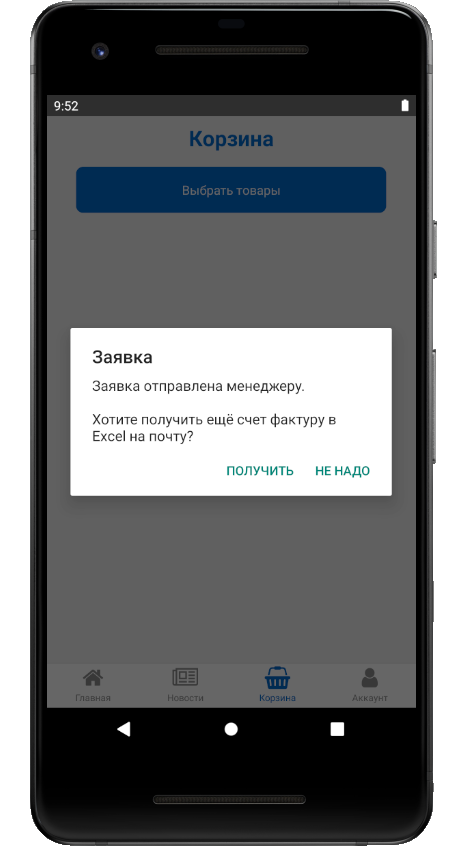
\includegraphics[height=6cm]
        {images/mobile/order/order-make.png}
    \end{minipage}
    \begin{minipage}{0.24\textwidth}
        \centering

        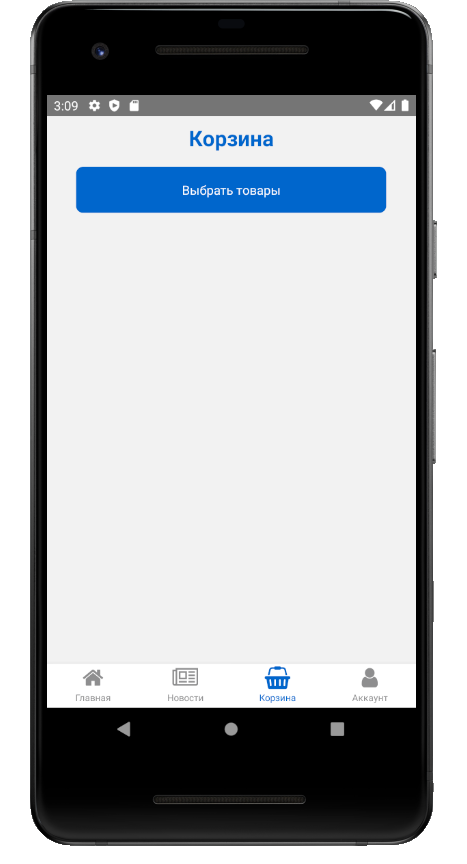
\includegraphics[height=6cm]
        {images/mobile/order/basket-empty.png}
    \end{minipage}

    \caption{Оформление заказа}
    \label{fig:test_order_make}
\end{figure}

\begin{figure}[!htb]\centering
    \begin{minipage}{0.24\textwidth}
        \centering

        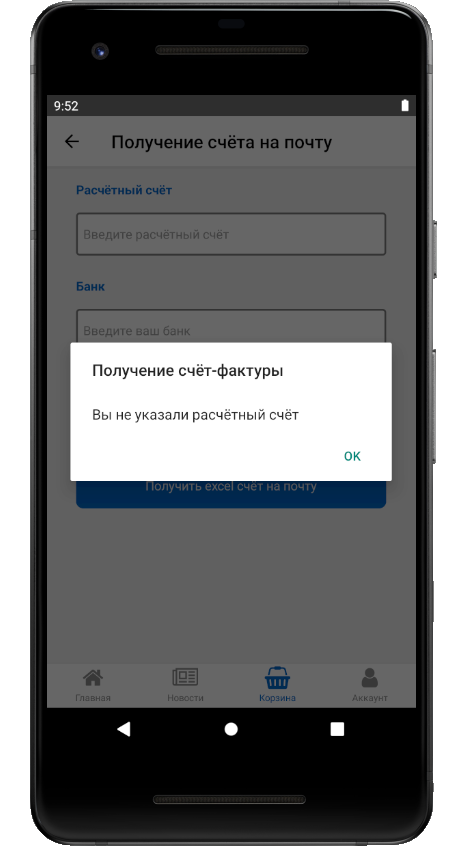
\includegraphics[height=6cm]
        {images/mobile/order/order-check-1.png}
    \end{minipage}
    \begin{minipage}{0.24\textwidth}
        \centering

        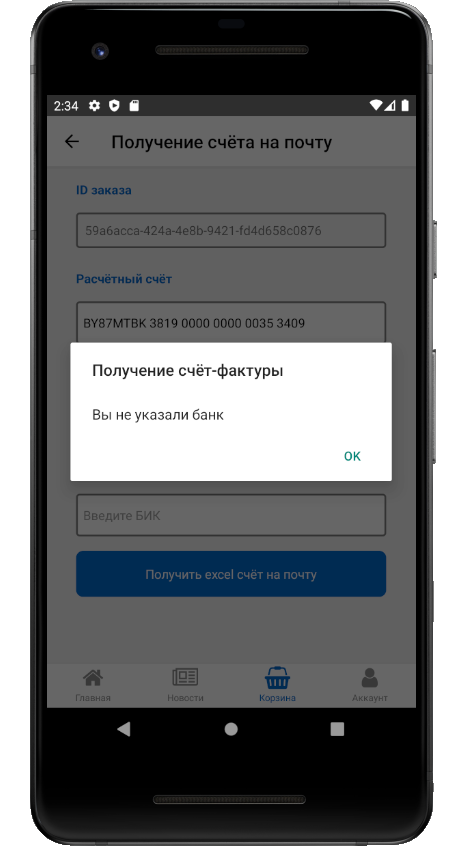
\includegraphics[height=6cm]
        {images/mobile/order/order-check-2.png}
    \end{minipage}
    \begin{minipage}{0.24\textwidth}
        \centering

        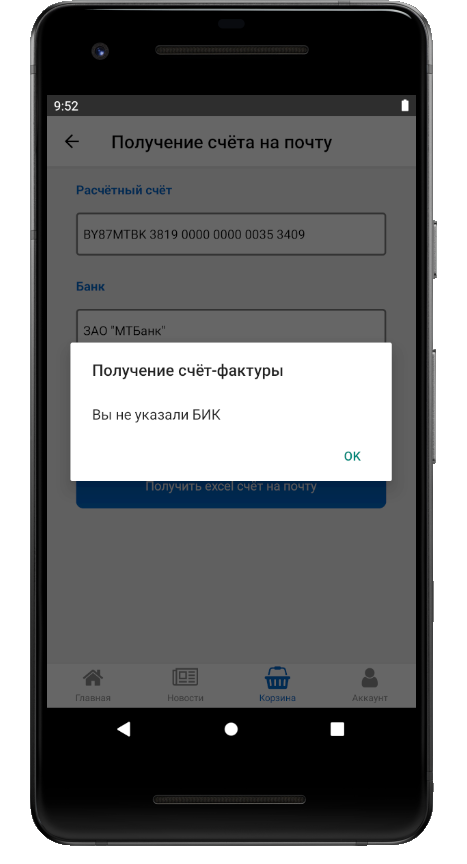
\includegraphics[height=6cm]
        {images/mobile/order/order-check-3.png}
    \end{minipage}
    \begin{minipage}{0.24\textwidth}
        \centering

        \includegraphics[height=6cm]
        {images/mobile/order/order-check-4.png}
    \end{minipage}

    \caption{Запрос счёт-фактуры с пустыми полями и заполнеными}
    \label{fig:test_order_check}
\end{figure}

\begin{figure}[!htb]\centering
    \begin{minipage}{0.25\textwidth}
        \centering

        \includegraphics[height=7cm]
        {images/mobile/order/order-email-1.png}
    \end{minipage}
    \begin{minipage}{0.25\textwidth}
        \centering

        \includegraphics[height=7cm]
        {images/mobile/order/order-email-2.png}
    \end{minipage}
    \begin{minipage}{0.25\textwidth}
        \centering

        \includegraphics[height=7cm]
        {images/mobile/order/order-email-3.png}
    \end{minipage}

    \caption{Сообщение с заказом и сообщение с Excel документом <<Счёт-факура>> на электронной почте}
    \label{fig:test_order_check}
\end{figure}

\begin{figure}[!htb]\centering

    \includegraphics[height=6.6cm]
    {images/mobile/order/order-email-4.png}

    \caption{Excel документ <<Cчёт-факура>> открытый в OnlyOffice}
    \label{fig:test_order_excel}
\end{figure}

Вывод:

\begin{itemize}
    \item[-] при отправки заявки корзина очистилась;
    \item[-] когда клиент не заполнил какое-нибудь поле, при отправки документа <<Счёт-фактура>>
    приложение отправило уведомление;
    \item[-] при успешной отправки заявки на e-mail пришло сообщение;
    \item[-] при успешном заполнении полей для документа <<Счёт фактура>> на электронную почту пришло сообщение,
    с прикрепленным Excel документом.
\end{itemize}

\subsection{Результаты испытания панели администратора}

\subsubsection*{Тест 1: Просмотр номенклатуры}

Ожидаемый результат: данные будут получены из БД и будут представлены в виде таблицы (см. рисунок~\ref{fig:test_admin_view}).
Кроме основных данных в таблице будут кнопки <<Обновить>> для перехода на страницу с формой для редактирования элемента и <<Удлаить>> для удаления элемента из БД.

\begin{figure}[!htb]\centering

    \includegraphics[width=18cm]
    {images/mobile/admin/tests/view_items.png}

    \caption{Отображение номенклатуры в виде таблицы}
    \label{fig:test_admin_view}
\end{figure}

Вывод: данные были получены с БД и отображены по колонкам в виде таблицы корректно.

\subsubsection*{Тест 2: Отображения формы для редактирования номенклатуры}

Ожидаемый результат: при нажатии кнопки <<Обновить>> появится страница с редактированием элемента,
на которой будет форма с заполнеными данными из БД.

Результат отображения данных в форме для редактирования номенклатуры изображен на рисунках \ref{fig:test_admin_item_edit_1} и \ref{fig:test_admin_item_edit_2}.

\begin{figure}[!htb]\centering

    \includegraphics[width=14cm]
    {images/mobile/admin/tests/item_edit_1.png}

    \caption{Отображение номенклатуры для редактирования}
    \label{fig:test_admin_item_edit_1}
\end{figure}

\begin{figure}[!htb]\centering

    \includegraphics[width=14cm]
    {images/mobile/admin/tests/item_edit_2.png}

    \caption{Отображение табличной части характеристик}
    \label{fig:test_admin_item_edit_2}
\end{figure}

Вывод: отображения формы для редактирования номенклатуры работает корректно.

\subsubsection*{Тест 3: Оповещение при удалении элемента}

Ожидаемый результат: при нажатии кнопки <<Удалить>> появится оповещение о том, что элемент будет удален.
Для продожения удаления кнопка <<Удалить>>, для отмены удаления - кнопка <<Не удалять>>.

Оповещение при удалении элемента отображено на рисунке~\ref{fig:test_admin_item_on_delete}.

\begin{figure}[!htb]\centering

    \includegraphics[width=14cm]
    {images/mobile/admin/tests/item_on_delete.png}

    \caption{Оповещение при кдалении элемента}
    \label{fig:test_admin_item_on_delete}
\end{figure}

Вывод: при нажатии кнопки <<Удалить>> появляется окно с предложением о продолжении удалении, либо её отмены.
При отказе от удаления, элемент не удаляется. Оповещение при удалении элемента работает корректно.

\subsection{Результаты испытания панели менеджера}

\subsubsection*{Тест 1: Вывод списка оставленных заявок}

Ожидаемый результат: заявки будут представлены в виде таблицы,
в которой можно увидеть сколько времени назад она была оставлена,
в которой указано количество выбранных позиций,
и в которой кнопка <<Просмотреть>> (см. рисунок~\ref{fig:test_manager_orders_view}).

\begin{figure}[!htb]\centering

    \includegraphics[width=18cm]
    {images/mobile/manager/tests/orders_view.png}

    \caption{Список оставленых заявок}
    \label{fig:test_manager_orders_view}
\end{figure}

Вывод: заявки отображаются в виде таблицы,
в которой текстом прописано сколько времени назад была оставлена заявка,
в которой указано количество позиций,
и в которой есть кнопка для просмотра заявки.
Отображение таблицы заявок работает корректно.

\subsubsection*{Тест 2: Отображение одной заявки}

Ожидаемый результат: на странице будут данные о заявке, о пользователе и список заказаной номенклатуры.

\begin{figure}[!htb]\centering

    \includegraphics[width=14cm]
    {images/mobile/manager/tests/order_view.png}

    \caption{Просмотр данных заявки}
    \label{fig:test_manager_order_view}
\end{figure}

Вывод: на странице одной заявки выведены данные о самой заявке, о пользователе и о заказаной номенклатуре.
Страница одной заявки отображается корректно.
